\documentclass{standalone}
\usepackage{tikz}
\usetikzlibrary{patterns, positioning}


\begin{document}
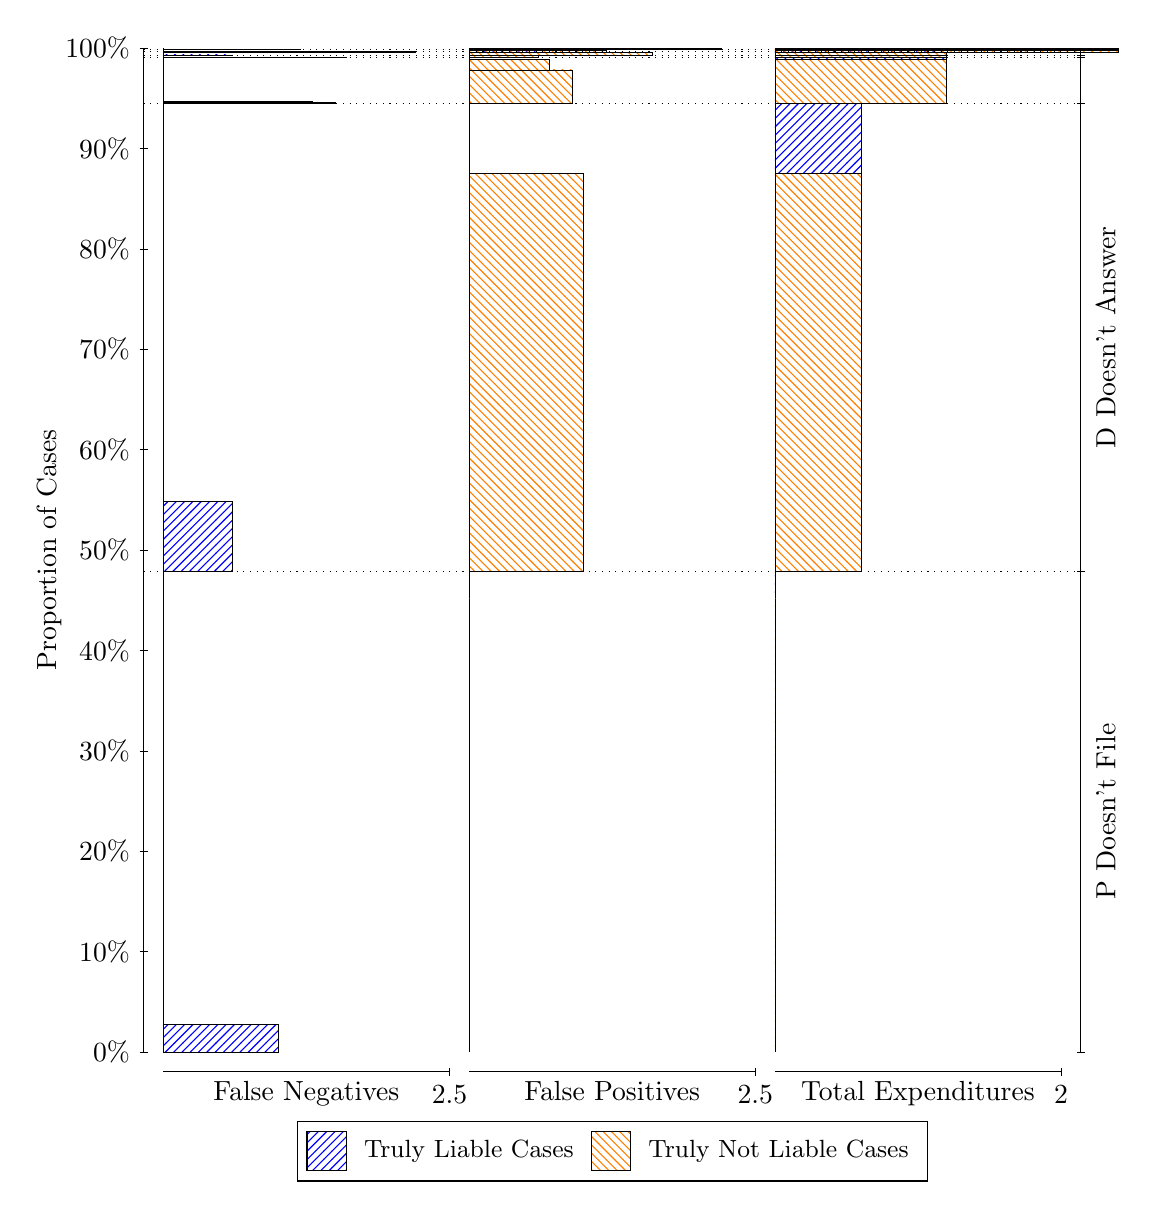
\begin{tikzpicture}
\draw[black, very thin] (1.5,1.75) -- (1.5,14.5);
\node[rotate=90, text=black, anchor=center] at (0.3, 8.125) {Proportion of Cases};
\draw[black, very thin] (1.45,1.75) -- (1.55,1.75);
\node[text=black, anchor=east] at (1.45, 1.75) {0\%};
\draw[black, very thin] (1.45,3.025) -- (1.55,3.025);
\node[text=black, anchor=east] at (1.45, 3.025) {10\%};
\draw[black, very thin] (1.45,4.3) -- (1.55,4.3);
\node[text=black, anchor=east] at (1.45, 4.3) {20\%};
\draw[black, very thin] (1.45,5.575) -- (1.55,5.575);
\node[text=black, anchor=east] at (1.45, 5.575) {30\%};
\draw[black, very thin] (1.45,6.85) -- (1.55,6.85);
\node[text=black, anchor=east] at (1.45, 6.85) {40\%};
\draw[black, very thin] (1.45,8.125) -- (1.55,8.125);
\node[text=black, anchor=east] at (1.45, 8.125) {50\%};
\draw[black, very thin] (1.45,9.4) -- (1.55,9.4);
\node[text=black, anchor=east] at (1.45, 9.4) {60\%};
\draw[black, very thin] (1.45,10.675) -- (1.55,10.675);
\node[text=black, anchor=east] at (1.45, 10.675) {70\%};
\draw[black, very thin] (1.45,11.95) -- (1.55,11.95);
\node[text=black, anchor=east] at (1.45, 11.95) {80\%};
\draw[black, very thin] (1.45,13.225) -- (1.55,13.225);
\node[text=black, anchor=east] at (1.45, 13.225) {90\%};
\draw[black, very thin] (1.45,14.5) -- (1.55,14.5);
\node[text=black, anchor=east] at (1.45, 14.5) {100\%};

\draw[black, very thin] (13.4,1.75) -- (13.4,14.5);
\draw[black, very thin] (13.35,1.75) -- (13.45,1.75);
\node[anchor=west] at (13.35, 1.75) {};
\draw[black, very thin] (13.35,7.856) -- (13.45,7.856);
\node[anchor=west] at (13.35, 7.856) {};
\draw[black, very thin] (13.35,13.794) -- (13.45,13.794);
\node[anchor=west] at (13.35, 13.794) {};
\draw[black, very thin] (13.35,14.384) -- (13.45,14.384);
\node[anchor=west] at (13.35, 14.384) {};
\draw[black, very thin] (13.35,14.405) -- (13.45,14.405);
\node[anchor=west] at (13.35, 14.405) {};
\draw[black, very thin] (13.35,14.451) -- (13.45,14.451);
\node[anchor=west] at (13.35, 14.451) {};
\draw[black, very thin] (13.35,14.479) -- (13.45,14.479);
\node[anchor=west] at (13.35, 14.479) {};
\draw[black, very thin] (13.35,14.5) -- (13.45,14.5);
\node[anchor=west] at (13.35, 14.5) {};

\draw[black, very thin, pattern color=blue, pattern=north east lines] (1.75,1.75) rectangle (3.2033,2.0955);
\draw[black, very thin, pattern color=orange, pattern=north west lines] (1.75,2.0955) rectangle (1.75,7.856);
\draw[black, very thin, pattern color=blue, pattern=north east lines] (1.75,7.856) rectangle (2.622,8.7422);
\draw[black, very thin, pattern color=orange, pattern=north west lines] (1.75,8.7422) rectangle (1.75,13.794);
\draw[black, very thin, pattern color=blue, pattern=north east lines] (1.75,13.794) rectangle (3.93,13.81);
\draw[black, very thin, pattern color=blue, pattern=north east lines] (1.75,13.81) rectangle (3.6393,13.82);
\draw[black, very thin, pattern color=orange, pattern=north west lines] (1.75,13.82) rectangle (1.75,14.384);
\draw[black, very thin, pattern color=blue, pattern=north east lines] (1.75,14.384) rectangle (4.0753,14.386);
\draw[black, very thin, pattern color=orange, pattern=north west lines] (1.75,14.386) rectangle (1.75,14.405);
\draw[black, very thin, pattern color=blue, pattern=north east lines] (1.75,14.405) rectangle (2.622,14.414);
\draw[black, very thin, pattern color=orange, pattern=north west lines] (1.75,14.414) rectangle (1.75,14.451);
\draw[black, very thin, pattern color=blue, pattern=north east lines] (1.75,14.451) rectangle (4.9473,14.453);
\draw[black, very thin, pattern color=orange, pattern=north west lines] (1.75,14.453) rectangle (1.75,14.479);
\draw[black, very thin, pattern color=blue, pattern=north east lines] (1.75,14.479) rectangle (3.494,14.483);
\draw[black, very thin, pattern color=orange, pattern=north west lines] (1.75,14.483) rectangle (1.75,14.5);
\draw[black, very thin, pattern color=orange, pattern=north west lines] (5.6333,1.75) rectangle (5.6333,7.5105);
\draw[black, very thin, pattern color=blue, pattern=north east lines] (5.6333,7.5105) rectangle (5.6333,7.856);
\draw[black, very thin, pattern color=orange, pattern=north west lines] (5.6333,7.856) rectangle (7.0867,12.907);
\draw[black, very thin, pattern color=blue, pattern=north east lines] (5.6333,12.907) rectangle (5.6333,13.794);
\draw[black, very thin, pattern color=orange, pattern=north west lines] (5.6333,13.794) rectangle (6.9413,14.221);
\draw[black, very thin, pattern color=orange, pattern=north west lines] (5.6333,14.221) rectangle (6.6507,14.358);
\draw[black, very thin, pattern color=blue, pattern=north east lines] (5.6333,14.358) rectangle (5.6333,14.384);
\draw[black, very thin, pattern color=orange, pattern=north west lines] (5.6333,14.384) rectangle (6.5053,14.403);
\draw[black, very thin, pattern color=blue, pattern=north east lines] (5.6333,14.403) rectangle (5.6333,14.405);
\draw[black, very thin, pattern color=orange, pattern=north west lines] (5.6333,14.405) rectangle (7.9587,14.442);
\draw[black, very thin, pattern color=blue, pattern=north east lines] (5.6333,14.442) rectangle (6.5053,14.451);
\draw[black, very thin, pattern color=orange, pattern=north west lines] (5.6333,14.451) rectangle (7.3773,14.477);
\draw[black, very thin, pattern color=blue, pattern=north east lines] (5.6333,14.477) rectangle (5.924,14.479);
\draw[black, very thin, pattern color=orange, pattern=north west lines] (5.6333,14.479) rectangle (8.8307,14.496);
\draw[black, very thin, pattern color=blue, pattern=north east lines] (5.6333,14.496) rectangle (7.3773,14.5);
\draw[black, very thin, pattern color=orange, pattern=north west lines] (9.5167,1.75) rectangle (9.5167,7.5105);
\draw[black, very thin, pattern color=blue, pattern=north east lines] (9.5167,7.5105) rectangle (9.5167,7.856);
\draw[black, very thin, pattern color=orange, pattern=north west lines] (9.5167,7.856) rectangle (10.607,12.907);
\draw[black, very thin, pattern color=blue, pattern=north east lines] (9.5167,12.907) rectangle (10.607,13.794);
\draw[black, very thin, pattern color=orange, pattern=north west lines] (9.5167,13.794) rectangle (11.697,14.358);
\draw[black, very thin, pattern color=blue, pattern=north east lines] (9.5167,14.358) rectangle (11.697,14.384);
\draw[black, very thin, pattern color=orange, pattern=north west lines] (9.5167,14.384) rectangle (11.697,14.403);
\draw[black, very thin, pattern color=blue, pattern=north east lines] (9.5167,14.403) rectangle (11.697,14.405);
\draw[black, very thin, pattern color=orange, pattern=north west lines] (9.5167,14.405) rectangle (11.697,14.442);
\draw[black, very thin, pattern color=blue, pattern=north east lines] (9.5167,14.442) rectangle (11.697,14.451);
\draw[black, very thin, pattern color=orange, pattern=north west lines] (9.5167,14.451) rectangle (13.877,14.477);
\draw[black, very thin, pattern color=blue, pattern=north east lines] (9.5167,14.477) rectangle (13.877,14.479);
\draw[black, very thin, pattern color=orange, pattern=north west lines] (9.5167,14.479) rectangle (13.877,14.496);
\draw[black, very thin, pattern color=blue, pattern=north east lines] (9.5167,14.496) rectangle (13.877,14.5);
\draw[black, dotted] (1.5,7.856) -- (13.4,7.856);
\draw[black, dotted] (1.5,13.794) -- (13.4,13.794);
\draw[black, dotted] (1.5,14.384) -- (13.4,14.384);
\draw[black, dotted] (1.5,14.405) -- (13.4,14.405);
\draw[black, dotted] (1.5,14.451) -- (13.4,14.451);
\draw[black, dotted] (1.5,14.479) -- (13.4,14.479);
\draw[black, very thin] (1.75,1.5) -- (5.3833,1.5);
\node[text=black, anchor=north] at (3.5667, 1.5) {False Negatives};
\draw[black, very thin] (5.3833,1.45) -- (5.3833,1.55);
\node[text=black, anchor=north] at (5.3833, 1.45) {2.5};

\draw[black, very thin] (5.6333,1.5) -- (9.2667,1.5);
\node[text=black, anchor=north] at (7.45, 1.5) {False Positives};
\draw[black, very thin] (9.2667,1.45) -- (9.2667,1.55);
\node[text=black, anchor=north] at (9.2667, 1.45) {2.5};

\draw[black, very thin] (9.5167,1.5) -- (13.15,1.5);
\node[text=black, anchor=north] at (11.333, 1.5) {Total Expenditures};
\draw[black, very thin] (13.15,1.45) -- (13.15,1.55);
\node[text=black, anchor=north] at (13.15, 1.45) {2};

\node[text=black, centered, rotate=90] at (13.72, 4.803) {P Doesn't File};
\node[text=black, centered, rotate=90] at (13.72, 10.825) {D Doesn't Answer};






\draw (7.449999999999999,1.5) node[draw=none] (baseCoordinate) {};
\begin{scope}[align=center]
        \matrix[scale=0.5, draw=black, below=0.5cm of baseCoordinate, nodes={draw}, column sep=0.1cm]{
            \node[rectangle, draw, minimum width=0.5cm, minimum height=0.5cm, pattern color=blue, pattern=north east lines] {}; &
            \node[draw=none, font=\small, text=black] (B) {Truly Liable Cases}; &
            \node[rectangle, draw, minimum width=0.5cm, minimum height=0.5cm, pattern color=orange, pattern=north west lines] {}; &
            \node[draw=none, font=\small, text=black] (B) {Truly Not Liable Cases}; \\
            };
\end{scope}

\end{tikzpicture}
\end{document}